\documentclass[]{article}

\usepackage{amsmath}
\usepackage{graphicx}

%opening
\title{Homework 3}
\author{Marwan Kallal}

\begin{document}

\maketitle

\section{}
See Matlab code

\section{}
\subsection*{(a)}
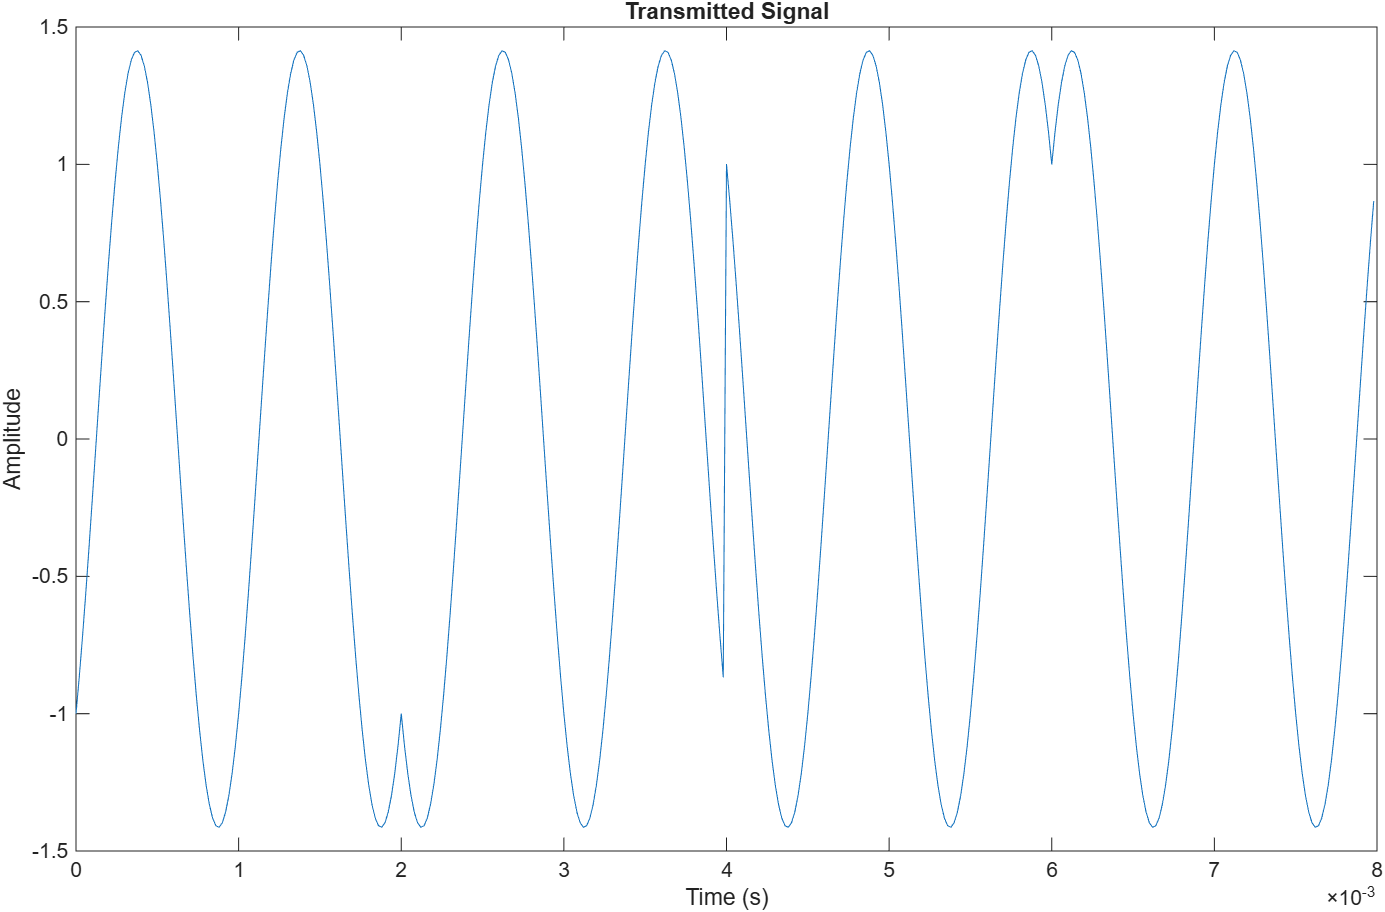
\includegraphics[width=\textwidth]{figures/tx_signal.png}\\
It is a PSK waveform, so the amplitude and frequency stay the same, and the phase shifts to represent different symbols (sets of bits). For example, the bits transmitted in this case are: $0,0,0,1,1,1,1,0$, and the first symbol (0,0) is at $225 \deg$, which matches the plot.

\subsection*{(b)}
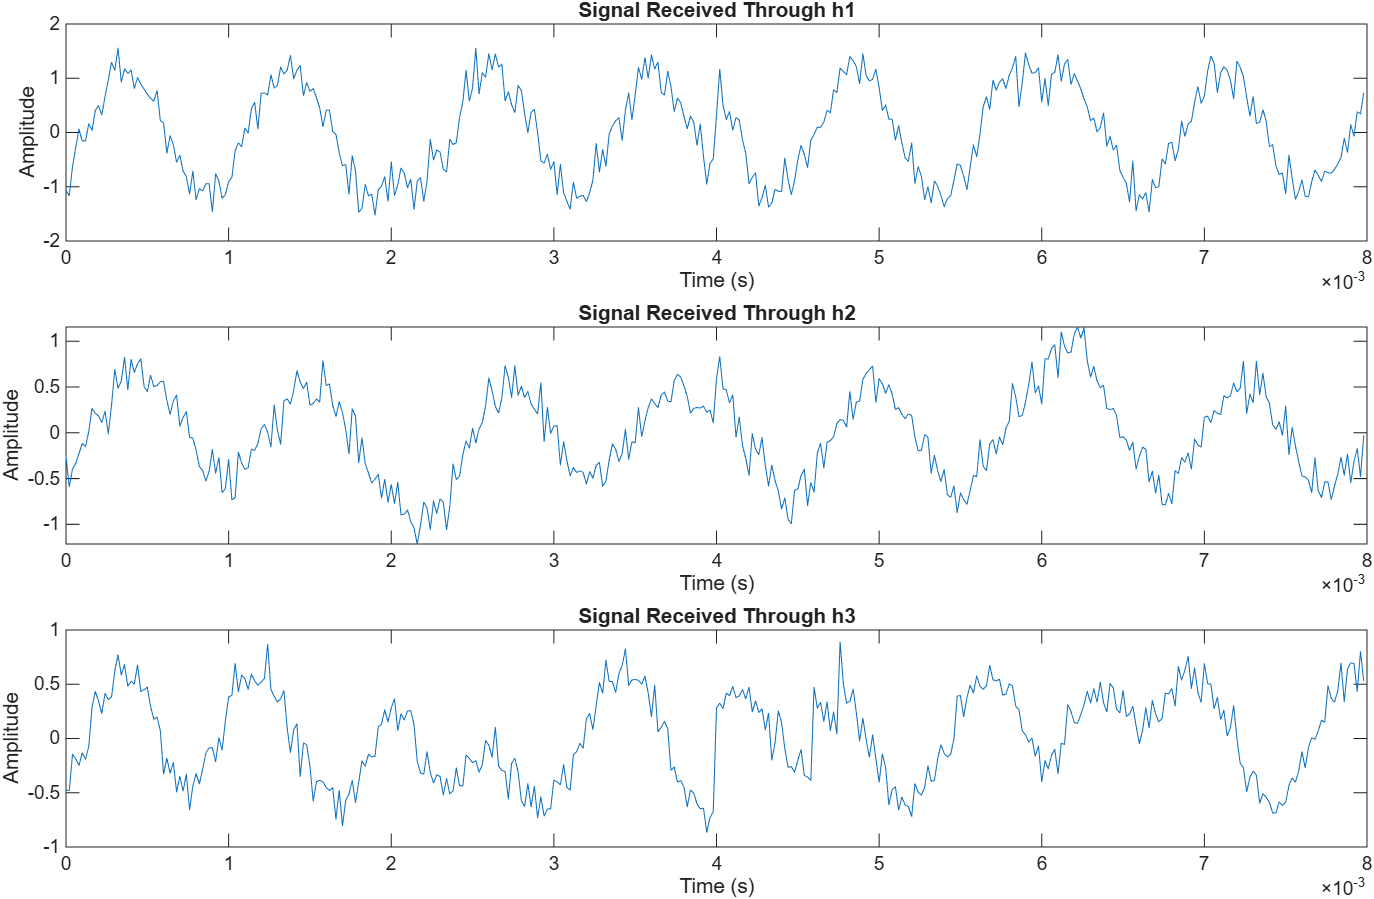
\includegraphics[width=\textwidth]{figures/rx_signals.png}\\
The distortion of the signal changes both the amplitude and phase of the signal. We can see in the h2 plot for example that most amplitude peaks are lower than in the undistorted signal due to the delayed copies destructively interfering. We can also see the distortion affect the phase, especially in the h3 plot, as at 2 seconds we expect to be near the negative peak of the sinusoid, but instead are half way through the positive side.\\
The h1 plot has only a single tap, and so only has AWGN but no distortion. The h2 plot has 3 taps, but h3 has 3 taps with higher delayed MPC power and longer delays, which causes more distortion in the signal. 

\section{}
\subsection*{(a)}
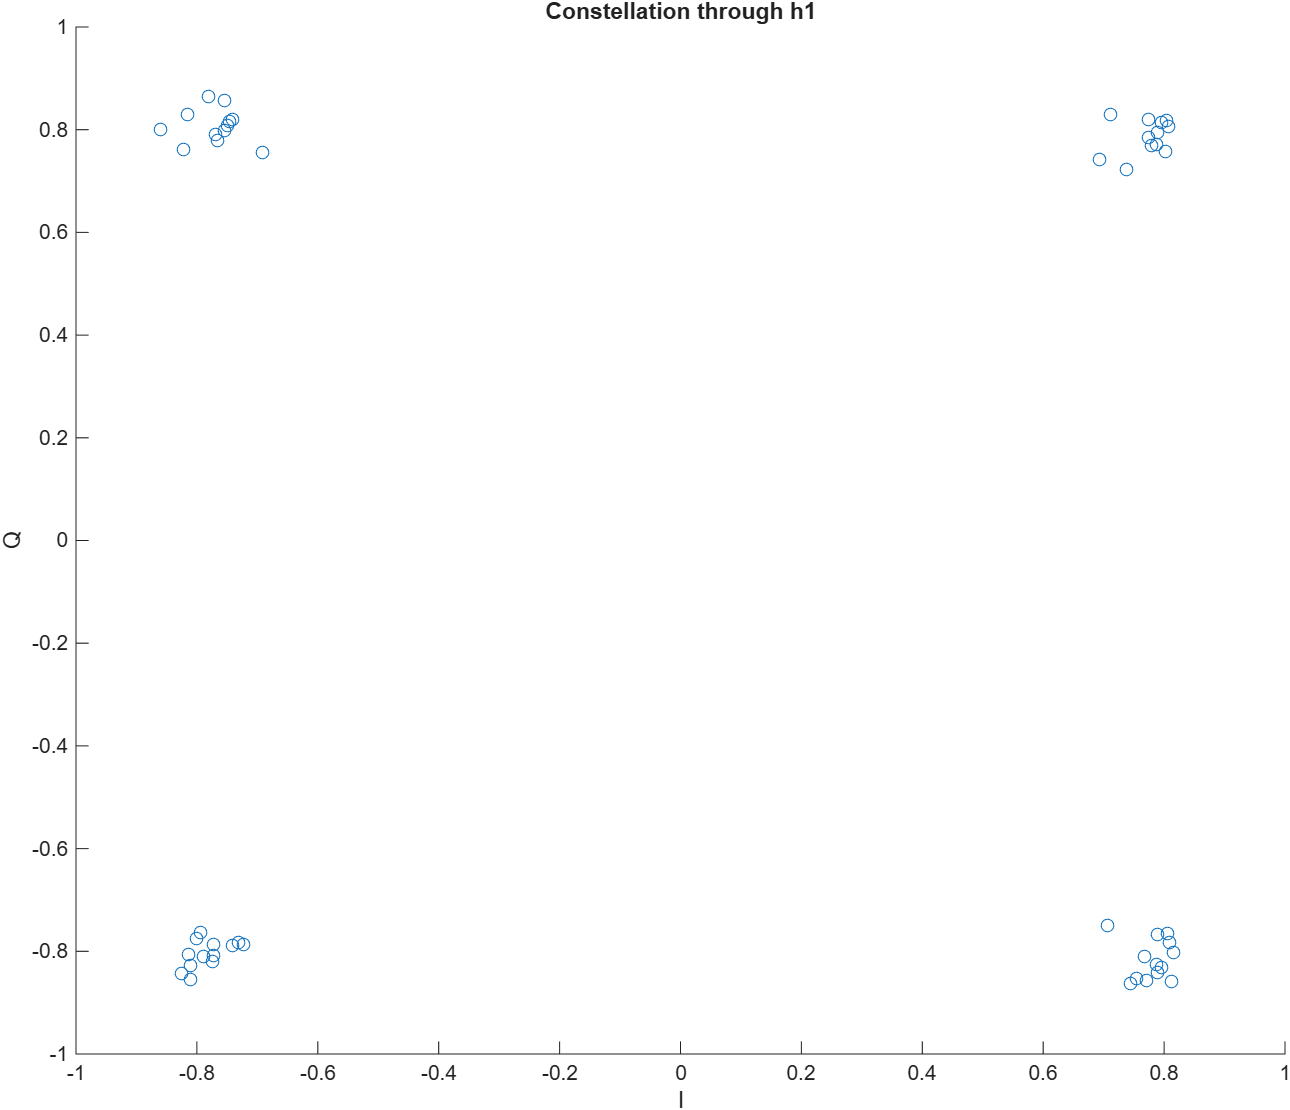
\includegraphics[width=\textwidth]{figures/constellation_h1.png}\\
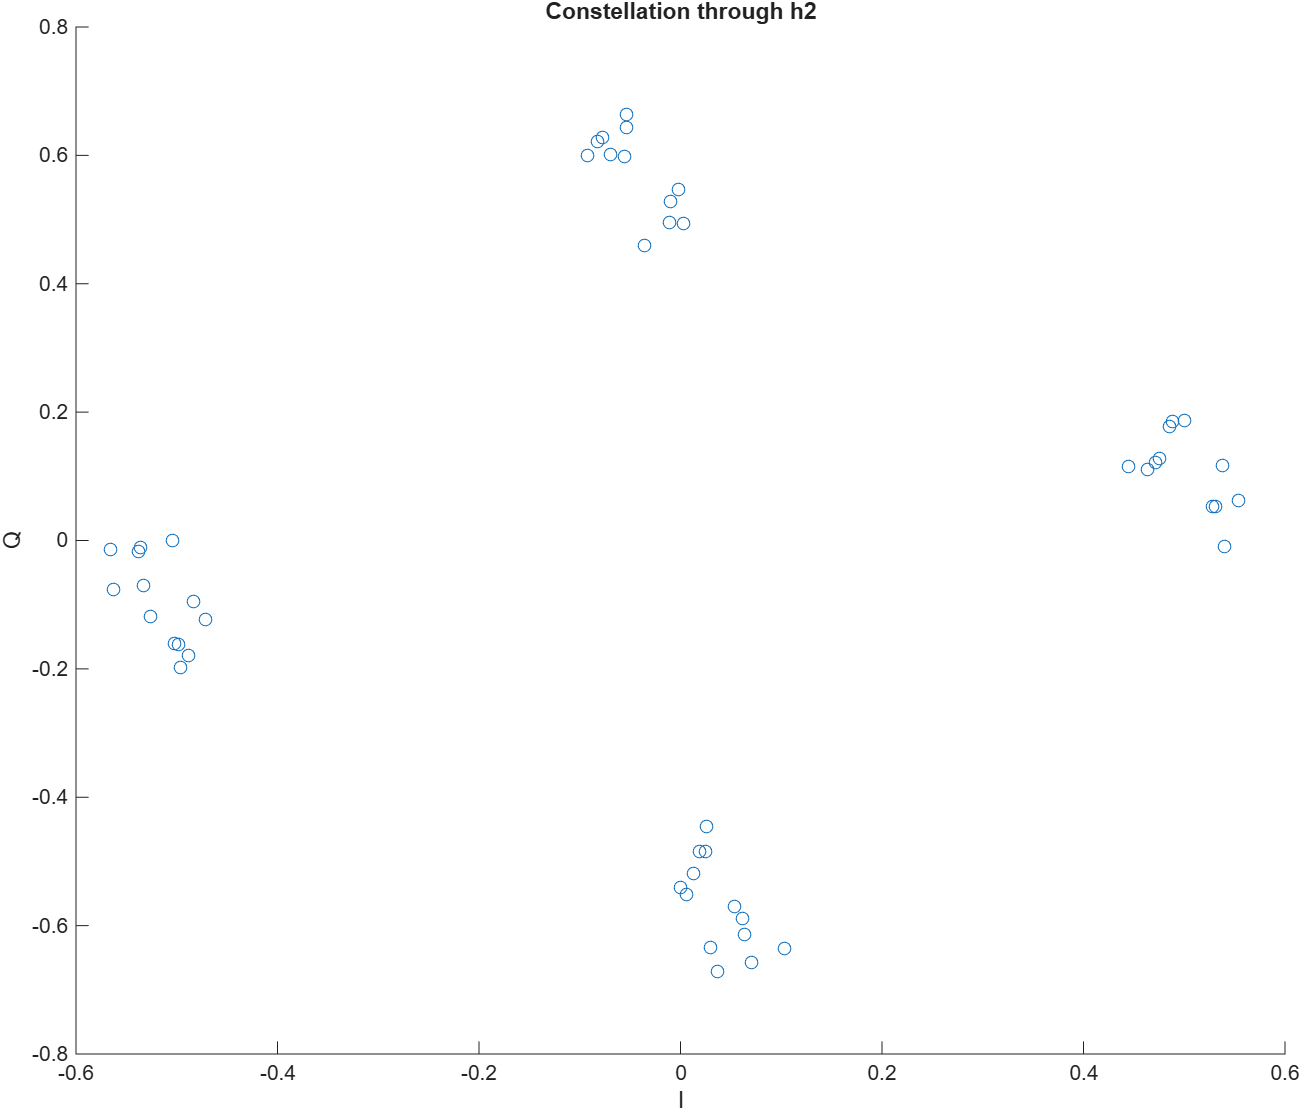
\includegraphics[width=\textwidth]{figures/constellation_h2.png}\\
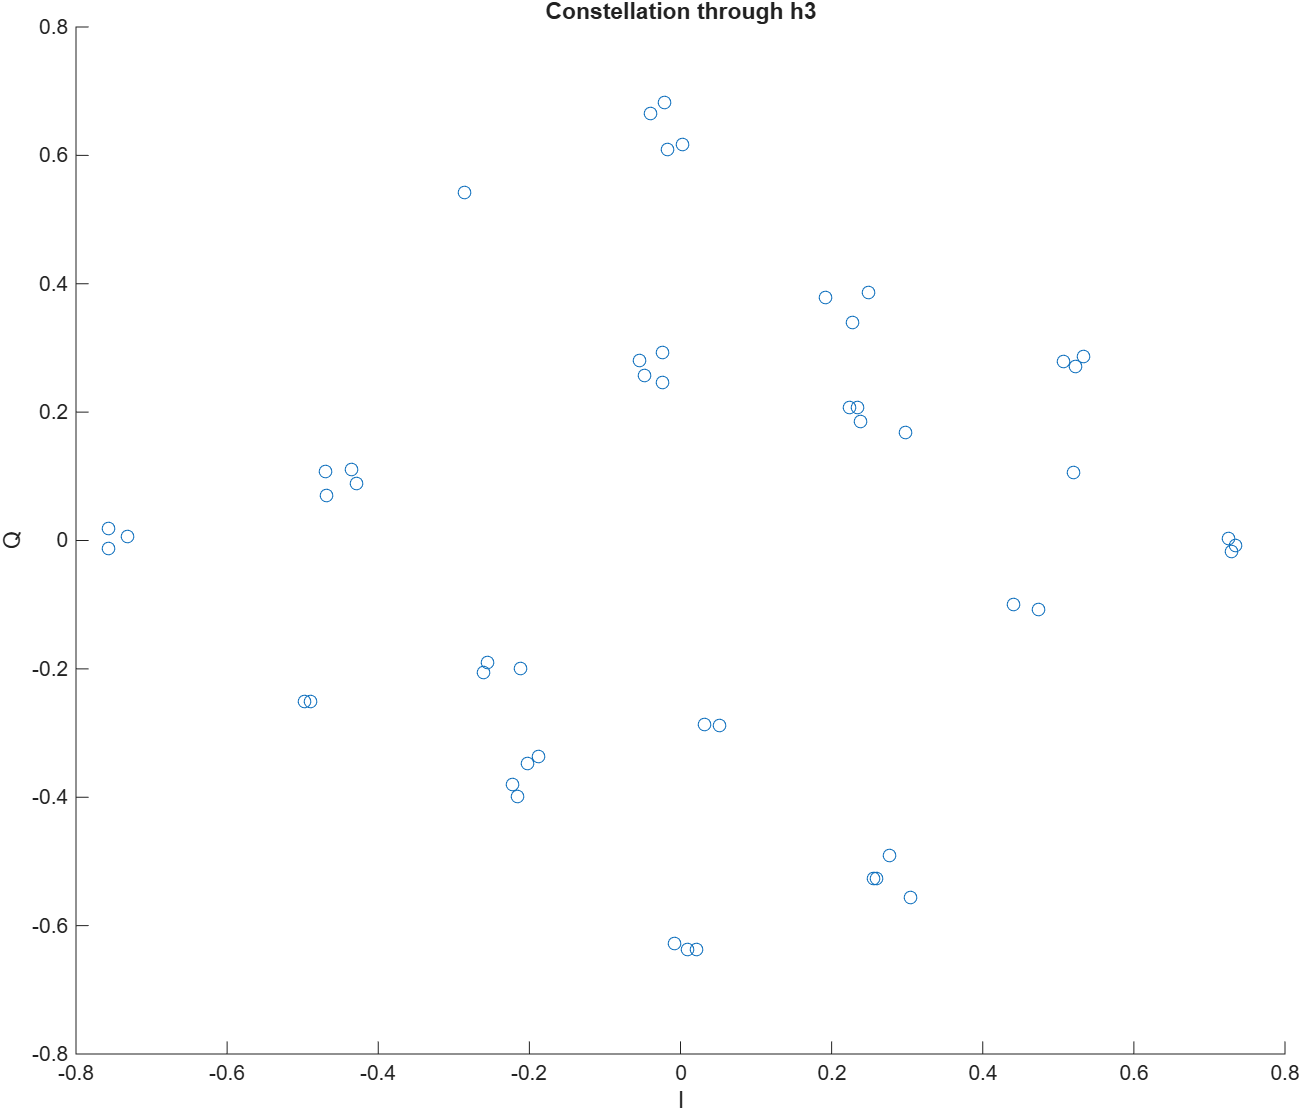
\includegraphics[width=\textwidth]{figures/constellation_h3.png}\\

The h1 plot shows a noisy signal with power of 0.8 (from the single tap). The h2 plot has a significant phase offset, with (at least visually) a larger variance in the clusters, but they stay around the same power, indicating flat fading. The h3 plot has significant fades and differing phase offsets across samples, without any clear constellation point clusters, likely coming from frequency selective fading because of our signal being wider than the coherence bandwidth.

\subsection*{(b)}
BER$_{h1} = 0$\\
BER$_{h2} = 0.03$\\
BER$_{h3} = 0.3$\\

h3 has the worst BER, likely because it has much longer delay spread (likely bringing our signal outside the coherence bandwith and causing frequency selective fading) and more power in the delayed MPCs, leading to (from the I/Q scatter plot) deep fades, and large phase shifts, preventing the receiver from recovering the symbols.

\section{}
I would use an equalizer to correct for the frequency selective fading. Likely MLSE since we are using a small constellation and it is optimal.

\section{}
\subsection*{(a)}
I did not use an AI tool, but when googling the "AI Summary" was present.
\subsection{(b)}
Searches such as "matlab rand", "matlab functions get outputs", "matlab size inputs must be integers".
\subsection{(c)}
I had originally said that h1 had constructive and destructive interference, having forgotten that it was a single tap channel, but after rechecking the channels in the assignment I corrected it.

\end{document}
